% !TeX root = ../main.tex
% Add the above to each chapter to make compiling the PDF easier in some editors.

\chapter{Methodology}\label{chapter:methodology}

% Describe creating dataset with blender, extracting synthetic data, adapting codes of each repositories, comparison, analysis, describe data visualization process (transfer functions)
In this chapter, we provide a detailed step-by-step of how we extracted depth values from our synthetic model and adapted the GS and MDE codes to accept synthetic data. We also provided our analysis and data visualization process in great detail. 

\section{Dataset Creation}

In this section, we explain how we selected a synthetic model and prepared it to be used for the training process of the 3DGS and MDE models.

\subsection{Model Selection}

\begin{figure}[h]
    \centering
    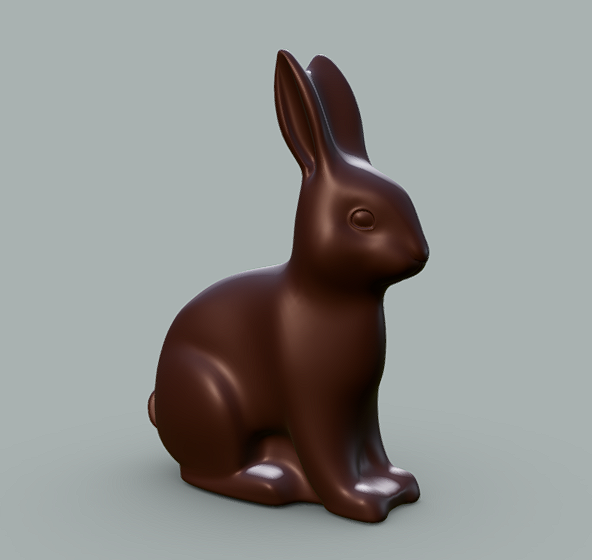
\includegraphics[width=0.5\linewidth]{figures/chocolate-easter-bunny.png}
    \caption{Chocolate Easter Bunny model by Louis Bidou}
    \label{fig:chocolate-bunny}
\end{figure}

Since this is an exploratory project aimed to test out different Gaussian Splatting models and pipelines, an object model had to be chosen to serve as an input for all the monocular depth estimation and Gaussian Splatting models being tested. A synthetic model is chosen since it is easier to gain Ground Truth data on it to be compared to the outputs of the models. In the interest of doing a simple evaluation to compare between depth values generated from the GS and depth estimation models, a simple object with not too many features and colors is chosen: the Chocolate Easter Bunny created by Louis Bidou (2015), licensed under CC BY 4.0 (see figure \ref{fig:chocolate-bunny}).

\subsection{Preprocessing with Blender}

\begin{figure}[h]
    \centering
    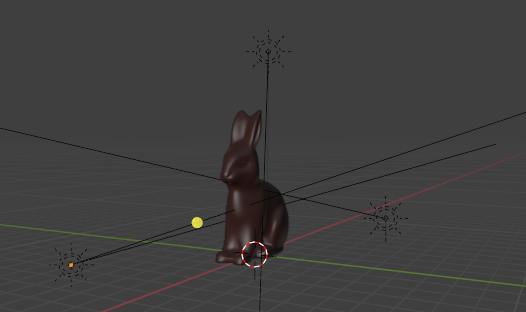
\includegraphics[width=0.5\linewidth]{figures/blender-showcase-01.png}
    \caption{Addition of lighting in Blender to illuminate the model}
    \label{fig:chocolate-bunny-blender}
\end{figure}

In order to compare the accuracy between models and also use this object model as an input for the monocular depth estimation and Gaussian Splatting models, the object model is first loaded inside Blender 4.3, an software for 3D modeling and simulations. Blender is chosen since it is a free and open-source software that has in-built Python scripting. Some lighting aimed at the Chocolate Bunny model is then added to illuminate the model's surrounding. This is done so that the model would have sufficient illumination during the rendering phase and would not appear dark. Proper illumination is needed to ensure that the training phase of each models would run well. 

\subsection{Extraction of Synthetic Depth Data (Ground Truth Data) and Input Dataset Creation from the Model}

Gaussian Splatting models require as input a collection of 2D images, along with its camera parameters. For this purpose, we create a Python script to process the model into a set of images to be used as input for the Gaussian Splatting models. The main goal of the script is to systematically take multiple images of the model following a spherical "grid" that surrounds the object and then save the images under a folder with a randomized name alongside with its camera parameters. This is done in order to capture the model from multiple different angles as best as possible while keeping the object in its entirety in the frame, so as not to produce a bad input that cannot be identified well by the Gaussian Splatting pipeline. Aside from storing images and camera parameters, the script also stores the absolute depth of each produced image in a separate folder. This allows us to view information of the ground truth depth map, which serves as a valuable point of evaluation for the Gaussian Splatting models. 

With this whole thing in mind, the script is created as follows: given two points in the Cartesian coordinate system, a box-like region of interest (where the object is located) is first identified, and from this, we are able to pinpoint the center of the object in the coordinate system. Afterwards, the \(x-, y-, z-\)Radius values of our spherical grid are calculated by looking at its difference to the extremes (the given input) of the box-like region. Next, the script requires two more input values to be specified to determine the number of images it needs to create as output: the number of "vertical steps" (height values) the spherical object will be divided into, and the number of captures (horizontal steps) we require per height values. In total, a number of \(vertical Steps \times horizontal Steps\) images are created. In the case of our Chocolate Bunny model, 6 different height values and 20 horizontal steps are specified, resulting in a total of 120 images.

Following this, we calculate the position of each camera. Each camera in principle is aimed at the center of the object, but they are placed in different locations according to the current height value and horizontal step combination. Hence, in order to calculate this, we do the following steps:
\begin{enumerate}
    \item We translate the object such that it lies in the center origin point of the Cartesian plane.
    \item We place an initial point a certain \(z-\)value length away from the center of the object. The length is calculated by considering the maximum value between the 3 different radius values calculated previously. We only consider the maximum value since our main goal is only to fit every part of the object into the camera frame. In the formula above, we also include a custom multiplier (to manually add some distance to the model), while the 'FoV' (Field of View) value is set according to the standard FoV in Blender (\(50.0^\circ\)).

    \begin{verbatim}
        maxRad = max(xRadius, yRadius, zRadius)
        alpha = math.sin(FoV)
        maxDist = Multiplier * (maxRad / alpha) * math.sqrt(1 - \
            (alpha * alpha))
    \end{verbatim}
    
    \item We rotate the point around the \(y-\)Axis for \(180.0^\circ/(heightValue + 1)\).
    \item We rotate the point around the \(z-\)Axis for \(360.0^\circ/(horizontalStep)\).
\end{enumerate}

Afterwards, it is only a matter of saving the resulting images inside the specified folder, alongside with its camera parameters and depth information (to serve as GT). The structure of the resulting output can be seen in figure \ref{fig:blender-structure}. In this way, we have achieved our original goal of producing a set of input images for our Gaussian Splatting models and, along with it, saved the ground truth depth images to serve as a point of reference.

\begin{figure}
    \centering
    \begin{center}
    \begin{forest}
    for tree={
        font=\ttfamily,
        grow'=0,
        child anchor=west,
        parent anchor=south,
        anchor=west,
        calign=first,
        edge path={
        \noexpand\path [draw, \forestoption{edge}]
        (!u.south west) +(7.5pt,0) |- node[fill,inner sep=1.25pt] {} (.child anchor)\forestoption{edge label};
    },
    before typesetting nodes={
      if n=1
        {insert before={[,phantom]}}
        {}
    },
    fit=band,
    before computing xy={l=15pt},
    }
    [randomName
        [depth
            [depth...]
            [...]
        ]
        [train
            [image...]
            [...]
        ]
        [camera\_center.json]
        [camera\_lookat.json]
        [transforms\_train.json]
    ]
    \end{forest}
    \end{center}
    \caption{File structure of the result of the Blender script for Dataset Preparation}
    \label{fig:blender-structure}
\end{figure}

\section{Code Adaption}

In order to ensure that the code runs perfectly on the synthetic data we produced from our Blender script, tiny adaptations are made in the code of each of the models we employed in this research.

The traditional 3DGS pipeline \parencite{3DGS} originally only accepts inputs that have been inserted into COLMAP (see Figure \ref{fig:colmap-structure}). This needed to be adjusted since reinserting our rendered images once more to COLMAP serves no purpose when we essentially already have everything that is needed and asked for by the 3DGS pipeline (e.g. transformation matrix, Field of Vision (FoV) values, camera angles). Therefore, some changes were made to the dataset\_reader\.py file of 3DGS to convert the camera information saved by Blender 4.3 into the format demanded by 3DGS to force it to accept synthetic information.

Similarly to how this is done in 3DGS, we also adapt the dataset reader files of 2DGS, RaDe-GS, GS2Mesh, ZoeDepth, and DepthAnything (both v1 and v2). Code adaptions and other scripts used in this thesis is made available in the following github repository: https://github.com/evelynsidarta/gaussian-splatting-thesis.

\begin{figure}[h]
    \centering
    \begin{center}
    \begin{forest}
    for tree={
        font=\ttfamily,
        grow'=0,
        child anchor=west,
        parent anchor=south,
        anchor=west,
        calign=first,
        edge path={
        \noexpand\path [draw, \forestoption{edge}]
        (!u.south west) +(7.5pt,0) |- node[fill,inner sep=1.25pt] {} (.child anchor)\forestoption{edge label};
    },
    before typesetting nodes={
      if n=1
        {insert before={[,phantom]}}
        {}
    },
    fit=band,
    before computing xy={l=15pt},
    }
    [inputFolder
        [images
            [image 0]
            [image 1]
            [...]
        ]
        [sparse
            [0 
                [cameras.bin]
                [images.bin]
                [points3D.bin]
            ]
        ]
    ]
    \end{forest}
    \end{center}
    \caption{File structure expected by the COLMAP loader of 3DGS}
    \label{fig:colmap-structure}
\end{figure}

\section{Training Process}

Training is done using the slightly-adapted code cloned from the respective github repositories of each model. For the number of training iterations, each model's number of training iterations is fixed at 10000 in order to give a fair evaluation when compared to each other. After the training is done, similar to gs2mesh, we render each outcome using the renderer script from 2DGS, since it also renders the depth map with the same camera poses as the original training images as a byproduct, which makes it a lot easier to do the evaluation step and compare the rendered outcome to the ground truth. The same number of images are therefore taken from the output model (120) after the rendering step.

\section{Evaluation Methodology}

\subsection{Data Postprocessing}

Since there might be slight differences in the output format of each model, some adjustments needed to be applied to the depth values of the outcomes of each model. To uniformize the outcome, it was decided that all of the depth map should be converted to inverted depth maps, which means that infinite depth (or empty spaces) will result in a depth value of 0, and objects that appear nearer to the camera will have a higher depth value when compared to objects that are farther away. Inverted depth maps have an advantage of having better numerical stability when compared to normal depth maps, especially for our Chocolate Easter Bunny model, since it has no background and comparing infinite values will only jeopardize the evaluation metrics. In order to invert the depth value, the following formula is applied to the resulting depth value outcomes:

\begin{center}
    \(x' = \frac{1}{x + \epsilon}\),
\end{center}
with \(x\) as the original value of the outcome, \(x'\) as the new inverted value, and \(\epsilon = 10^{-3}\), which is a small margin that is added to prevent division by zero. Overall, depth inversion is applied to the ground truth images, as well as 3DGS, 2DGS, ZoeDepth, RaDe-GS, and GS2Mesh images. This depth inversion is not applied to the DepthAnything v1 and v2 outcome images since they are already inverted from the start. 

Other than depth inversion, normalization using min-max scaling is also applied to all the outcome images in order to generalize the outcome values to be comparable. Normalization is done with the following formula:

\begin{center}
    \(x' = \frac{x - x_{min}}{x_{max} - x_{min}}\),
\end{center}
with \(x_{min}\) as the current lowest value of the depth map (the background value, since it is fixed at 0) and \(x_{max}\) as the current highest value in the depth map.

\subsection{Evaluation Metrics}

In order to provide a thorough analysis of the depth results of the rendered models, and inspired by the evaluation method of ZoeDepth \parencite{ZoeDepth}, each of the 120 depth images from the outcome are compared to the ground truth depth values and the following error metrics are calculated and averaged for each model: 1) Scale Invariant Logarithmic (SiLog) loss, 2) Threshold accuracy \((\delta_1, \delta_2, \delta_3)\), 3) Root Mean Squared Error (RMSE), 4) Root Mean Squarde Log Error (RMSLE), 5) Absolute Relative Error (REL), 6) Logarithmic Error, and 7) Relative Square Error (RSE).

\subsubsection{Absolute Relative Error (REL)}

Absolute Relative Error (REL) measures the absolute difference between the predicted and the ground truth depth value when compared to the ground truth depth value. Absolute Relative Error is calculated as follows:

\begin{center}
    REL = \(\frac{1}{M} \sum\limits_{i = 1}^{M} \frac{|d_i - \hat{d_i}|}{\hat{d_i}}\),
\end{center}
with \(d_i\) as predicted depth value at the \(i\)-th pixel, \(\hat{d_i}\) as ground truth depth value at the \(i\)-th pixel and \(M\) as the total amount of pixels. A lower REL value generally indicates better performance.

\subsubsection{Scale Invariant Logarithmic Loss}

Scale Invariant Log loss (SiLog) is a metric often used to evaluate Monocular Depth Estimation models. MDE is an ill-posed problem, which means that there is an infinite amount of geometrical solutions due to scaling. Therefore, SiLog loss function is created to minimize the impact of this scaling problem and only consider relative error in the logarithmic space instead of directly comparing absolute values. The formula for SiLog error is as follows:

\begin{center}
    SiLog \(= \sqrt{\frac{1}{M} \sum\limits_{i = 1}^{M}(\ln d_i - \ln \hat{d_i})^2 - \frac{1}{M^2} (\sum\limits_{i = 1}^{M} (\ln d_i - \ln \hat{d_i}))^2}\),
\end{center}
with \(d_i\) as the predicted depth value at the \(i\)-th pixel, \(\hat{d_i}\) as the ground truth value at the \(i\)-th pixel, and \(M\) as the total amount of pixels. SiLog value gets higher along with the value discrepancies, so a lower SiLog value is generally preferred.

\subsubsection{Threshold Accuracy}

Threshold accuracy typically evaluates how well the predicted depth map values align with the ground truth values. It measures the percentage number of pixels that are within a factor of \(\delta^n\) when compared to the ground truth values. The calculation for threshold accuracy is as follows:

\begin{center}
    \(\delta_n = \%\) of pixels that satisfy \(max (\frac{d_i}{\hat{d}_i}, \frac{\hat{d}_i}{d_i}) < \delta^n\) \parencite{ZoeDepth},
\end{center}
with \(d_i\) as predicted depth value at the \(i\)-th pixel and \(\hat{d_i}\) as ground truth depth value at the \(i\)-th pixel. The value of \(\delta\) is set to be 1.25, which means that \(\delta_1\) evaluates the percentage number of pixels whose value lie within 25\% of the ground truth value, while \(\delta_2\) and \(\delta_3\) respectively evaluate the number of pixels whose value lie between 56.25\% and 95.31\% of the value of the ground truth. For threshold accuracy, the closer the value is to 100\%, the better the performance of the evaluated model is, since it means that the predicted values are close to the values of the ground truth.

\subsubsection{Root Mean Squared Error (RMSE)}

Root Mean Squared Error (RMSE) is an error that describes absolute differences between ground truth values when compared to the predicted values. Here, high discrepancies are highlighted due to the squaring operation in the formula. RMSE is calculated as follows:

\begin{center}
    RMSE \(= \sqrt{\frac{1}{M} \sum\limits_{i = 1}^{M} (d_i - \hat{d_i})^2}\),
\end{center}
with \(d_i\) as predicted depth value at the \(i\)-th pixel, \(\hat{d_i}\) as ground truth depth value at the \(i\)-th pixel and \(M\) as the total amount of pixels. Since this metric value gets higher along with the value discrepancies, a lower RMSE value is generally preferred and indicate better performance. 

\subsubsection{Root Mean Squared Logarithmic Error (RMSLE)}

Root Mean Squared Logarithmic Error works in a similar manner to RMSE, but the values are first log-transformed before being compared to the also-transformed ground truth value. RMSLE is useful to proportionally scale higher discrepancies compared to just taking the absolute difference calculation. RMSLE is measured as follows:

\begin{center}
    RMSLE \(= \sqrt{\frac{1}{M} \sum\limits_{i = 1}^{M} (\ln (d_i) - \ln (\hat{d_i}))^2}\),    
\end{center}
with \(d_i\) as predicted depth value at the \(i\)-th pixel, \(\hat{d_i}\) as ground truth depth value at the \(i\)-th pixel and \(M\) as the total amount of pixels. Similarly to RMSE, a lower RMSLE value is preferred during evaluation.

\subsubsection{Logarithmic Error}

Logarithmic error measures the log-transformed difference between the predicted and ground truth depth values. Logarithmic error is measured as follows:

\begin{center}
    Log Error = \(\frac{1}{M} \sum\limits_{i = 1}^{M} |\log_{10} (d_i) - \log_{10} (\hat{d_i})|\),
\end{center}
with \(d_i\) as predicted depth value at the \(i\)-th pixel, \(\hat{d_i}\) as ground truth depth value at the \(i\)-th pixel and \(M\) as the total amount of pixels. A lower logarithmic error value indicates better model performance.

\subsubsection{Relative Square Error (RSE)}

Relative Square Error (RSE) works similarly to absolute relative error, but instead of calculating absolute difference it squares the result, which means that it magnifies error values more. RSE is calculated as follows:

\begin{center}
    RSE = \(\frac{1}{M} \sum\limits_{i = 1}^{M} \frac{(d_i - \hat{d_i})^2}{\hat{d_i}^2}\),
\end{center}
with \(d_i\) as predicted depth value at the \(i\)-th pixel, \(\hat{d_i}\) as ground truth depth value at the \(i\)-th pixel and \(M\) as the total amount of pixels. A lower RSE indicates better performance.

\section{Data Display}

Aside from statistical evaluation, we also compare the results of each model visually. In order to do this, samples from each models are gathered and compared side-by-side to each other with pyplot. For all the depth maps except for the Depth Anything models, the depth is inverted, similarly to how it is done during evaluation process. For 3DGS, RaDe-GS, and GS2Mesh, aside from the usual depth map inversion to uniformize the depth maps, the sigmoid transfer function is applied. This is done in order to better show the differences in values, since these three depth maps have only very slight differences between values inside the depth map.

\subsection{Sigmoid Transfer Function}

Sigmoid transfer function is commonly used to address the vanishing gradient problem: when inputs are too extreme, it is often hard to see tiny changes in the value. The sigmoid transfer function addresses this problem by compressing extreme values in an image and expanding the middle range of the values. Values after applying the sigmoid transfer function is calculated as follows:

\begin{center}
    \(\sigma(x) = \frac{1}{1 + e^{-k \cdot (x - x_0)}}\),
\end{center}
with \(x_0\) as the "middle range" we are trying to expand and k as the steepness of the sigmoid curve.